\section*{Proposition}
\subsection*{Introduction}
\paragraph{}
L'annotation d'un triplet RDF est une façon d'ajouter des metadonnées à un triplet RDF pour décrire la validité temporelle, une restriction spatiale, ect...
\newline
\textit{Comment on utilise les annotations temporelles ?}
Sur le site sig.ma\footnote{http://sig.ma/} créer par\textit{the digital enterprise research institute in Ireland}, la plateforme fournit un moteur de recherche par mot clé qui permet de récupérer des images et des textes accessibles par des annotations RDF, ainsi que d'une liste d'URI synonymes correspondant à la clé de recherche et des liens vers des sources Web contenant des données RDF pertinentes.
\subsection*{Schéma de modélisation}
\paragraph{}
Notre première modélisation a été conçu de la manière suivante :
\newline
Tout d’abord, et à partir des différents sources d’informations on veut récupérer les informations temporelles dans leurs contextes sémantiques à l’aide de nos différents extracteurs implémentés. 
Ensuite, les mettre dans un ensemble de fichiers comme le montre le schéma ci-dessous.
\begin{figure}[H]
        \centering
                \centering
                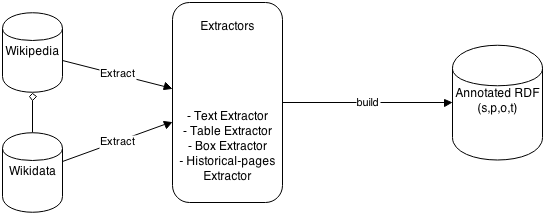
\includegraphics[width=10cm]{modelisation.png}
               \caption{Modélisation générale}

\end{figure}
\subparagraph{}
Certes, on peut créer des “patterns” partons ou motifs à travers les faits temporels dans la base de connaissances mais on cherche ici à extraire les informations des textes et des données semi-structurée afin de leur trouver une autre structure plus adéquate (tel un triplet annoter ou bien un quadrupet).
\subsection*{Démarche}
\paragraph{}
Au début, nous avons commencé par une procédure d’extraction classique avec un parseur avec l'API SAX pour extraire des données temporelles des dumps xml de wikipédia. Nous avons réussi à extraire plusieurs informations temporelles mais nous avons rencontré des problèmes relatives à la taille du dumps wikipédia/wikidata et au fait de relier ces informations temporelles au bon contexte du triplet qu’on veut annoté.
\subparagraph{}
Ce fait nous a amené à chercher une autre solution que celle choisi au départ.
Nous avons trouvé une solution plus intelligente pour former les quads ou des triplets annotés à partir des dumps DBpedia.
\subparagraph{}
Sur le site de DBpedia, nous avons étudié les deux formats du dumps JSON et CSV afin de voir la structure des informations.
Suite à nos observations nous avons décidé de manipuler les fichiers CSV pour voir la logique et la structure de ces informations.
\subparagraph{}
Nous cherchons à former les quadruplets à partir des faits existants dans DBpedia.
Dans cette dernière, on trouve des faits temporels et d’autres faits relié à leurs contexte.
\subparagraph{}
Une liste des faits sera proposer en output et un expert sera placer pour juger la validité des données trouvées par notre algorithme sous forme de résultats labellisés en premier temps puis d'enregistrer les ressources dans des fichiers de quadruplets RDF classés selon des catégories bien spécifiques.
L’expert peut sélectionner la liste des indicateurs $tokens$ temporels misent par défaut dans le code de l’application, ajouter des indicateurs à la liste existante ou bien introduire une nouvelle liste d’indicateurs.
Sachant que plus on introduit des indicateurs temporels, plus on aura des couples.
\subparagraph{}
Nous avons testé notre algorithme avec les deux indicateurs $YEAR$ et $DATE$.
L'algrithme cherche à trouver une liste de couple de faits temporels et faits reliés possible qui seront les entrées d'une requête $SPARQL$.
\subparagraph{}
L'expert intervient pour juger la validiter des résultats trouvés.
Un seul output valide peut donnée un ou plusieurs résultats ''des triplets annotés''.
Nous avons défini une base SPOTbase ($Subject$, $Predicate$, $Object$, $Time$) qui contient les quadruplets extraits par catégorie.
\subparagraph{}
Nos algorithmes manipulent des ressources DBpedia afin de les mettre sous un autre forme valide dans le temps et tout en gardant une sémantique correcte. 
\subsection*{Procédure}
\paragraph{}
Notre proposition consiste à extraire des faits temporels de la forme suivant :
\newline
$***Entity*with*TemporalToken***$ puis de chercher d’autres propriétés reliées à ces faits temporels $***Entity*with*OtherWord***$.
On donne la main à un expert pour choisir un couple de faits puis de valider les résultats générer automatiquement par notre algorithme afin de mettre en place les quadruplets dans la base SPOTbase. 
\subsubsection{Étapes}
\paragraph{}
La première étape consiste à trouver tout les propriétés et les stockers dans un fichier pour les exploités comme une base de faits.
\newline
Algorithme : getProperties(propFile)			
\newline
writer<=bufferWriter(propFile)
\newline
resultSet<=queryExecution(query)                         
\newline
writeProperties(resultSet,writer)				
\paragraph{}
L'étape suivante consiste à trouver la liste des faits temporels à partir de la liste d'indicateurs mise par défaut ou introduite par l'expert.
\newline
Algorithme : getTemporalFacts(tToken, propFile) 			
\newline
buff <= ReadFile(propFile)    			
\newline
tf<=ListFacts(buff,tToken) 				
\newline
removeDuplication(tf)
\paragraph{}
La procédure d'extraction continue pour extraire les faits reliés, à partir de la liste de faits temporels trouvés. On cherche à extraire un nombre maximal de faits reliés pour avoir plus de résultats.
\newline
Algorithme : findCouple  			
\newline
getPairListAtt(file,tf)
\newline
listToken<=findTokens(tf,tp)   
\newline      
hashSet<=getHashSetList(listToken) 
\newline
printList(hashSet)				
\paragraph{}
Le choix de l'expert consiste à selectionner le couple de faits pour lancer automatiquement l'algorithme qu'on a conçu permettant de récuperer les informations nécessaires pour former des triplets annotés.
\newline
Notre besoin se résume comme suit :
\newline
if ($x$ propTemp $y$) and ($x$ prop*** $z$) then
\newline
($x$ prop*** $z$) $y$ with ($y$ is the temporal annotation)
\subparagraph{}
Les résultats de la requête labelisés seront affichés dans un $TextArea$ à l'expert en premier lieu puis ils peuvent être stocker dans un fichier sous forme de quadruplets RDF.
Les quadruplets annotés seront sauvegardés dans le fichier nommé par l'expert dans le dossier de la base de donnée SPOTbase.
\subparagraph{}
Pour obtenir des quadruplets on a essayé de trouver des propriétés qui se rencontrent avec une procédure automatique mais le choix de l’expert et la validation des résultats à toujours important. Cela peu avoir un impacte déterminant sur le reste du travail et la nature des résultats.
\subsection*{Récapitulatif}
\paragraph{}
Nous avons construit à partir de la base de connaissance DBpedia une autre base de  triplets temporairement annotés qu’on a nommé SPOTbase.
SPOTbase contient une liste de fichiers dans lesquels on a des quadruplets ($subject$, $predicat$, $object$, $time$) avec une sémantique correcte. 
\subparagraph{}
Par la suite, nous avons choisi d’extraire des propriétés temporelles liées à une liste d'indicateurs pour tourner nos algorithmes.
\subparagraph{}
Une première étape consiste à extraire tous les faits DBpedia et les stockés dans un fichier puis la seconde consiste à proposer une liste de couple de faits à l’expert.
\subparagraph{}
Dans l’étape suivante on va interroger DBpedia en utilisant une requête SPARQL qui retourne trois variables ($x$,$y$,$z$) le choix de l’expert est primordiale pour valider les résultats trouvés.
Enfin les ressources formées en quadruplets seront stockés dans SPOTbase.   
\newline
( $X$ prop\_liée $Y$ ) annoté avec $Z$.
\subparagraph{}
Notre nouvelle approche à la particularité de manipule directement les ressources de DBpedia.
Des anciens travaux de recherches ont évoqué la même problématique en essayant de rattacher des annotions aux données de wikipedia alors que dans notre étude nous cherchons à regrouper des propriétés des triplets existants afin de former des triplets annotés.





		


 
